	\documentclass[twoside]{article}
\usepackage{../../estilo-ejercicios}
\setcounter{section}{0}
\newtheorem{defin}{Definition}[section]
\newtheorem{lem}[defin]{Lemma}
\newtheorem{propo}[defin]{Proposition}
\newtheorem{thm}[defin]{Theorem}
\newtheorem{eje}[defin]{Example}
\newtheorem{obs}[defin]{Observación}
\renewcommand{\baselinestretch}{1,3}
%--------------------------------------------------------
\begin{document}

\title{Characterization of Extremal Antipodal Polygons}
\author{Javier Aguilar Martín}
\maketitle

%\varprojlim
%\varinjlim
\section{Introduction}



\begin{defin}
A set of $2n$ ($n\geq 3$) points on the unit circle centered at the origin is called an \emph{antipodal point set} if for every point $p\in S$, also $p'\in S$. Let $S=\{p_1,p_1'\dots,p_n,p_n'\}$ such set. An \emph{antipodal polygon} on $S$ is a convex polygon  having as vertices one point from each pair $(p_i,p_i')$. A \emph{thin} antipodal polygon $P$ is an antipodal polygon whose verticies are consecutive points on the circle. For $n$ odd, a \emph{thick} antipodal polygon $P$ is an antipodal polygon such that there is a point of $S$ between every two vertices of $P$. For $n$ even there is exactly one pair of vertices of $P$ which are consecutive on the circle. 
\end{defin}

\begin{figure}[h!]
\centering
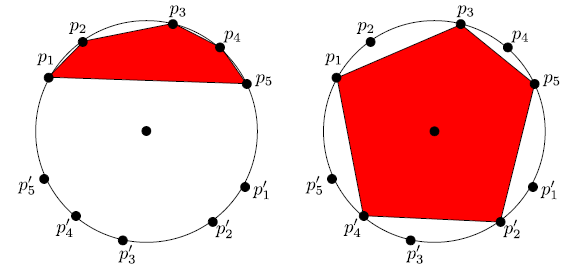
\includegraphics[scale=0.7]{fig1}
\caption{A thin (left) and a thick (right) antipodal polygon.}
\end{figure}

\definecolor{ffqqqq}{rgb}{1.,0.,0.}
\begin{figure}
\begin{tikzpicture}[line cap=round,line join=round,>=triangle 45,x=1.0cm,y=1.0cm]
\clip(-6.9,-2.533333333333284) rectangle (10.92,2.353333333333335);
\fill[line width=1.pt,color=ffqqqq,fill=ffqqqq,fill opacity=1.0] (-1.6937799777061364,1.063536265071295) -- (-0.7492357887671589,1.8543585771987179) -- (1.0656265393722786,1.6924656801795013) -- (1.7635692838693833,0.9433045006743214) -- (1.225143330871628,-1.5808301043504873) -- (0.,-2.) -- cycle;
\draw[line width=1.pt] (-1.6937799777061364,1.063536265071295) -- (-0.7492357887671589,1.8543585771987179) -- (1.0656265393722786,1.6924656801795013) -- (1.7635692838693833,0.9433045006743214) -- (1.225143330871628,-1.5808301043504873) -- (0.,-2.) -- cycle;
\draw [line width=1.pt] (0.,0.) circle (2.cm);
\draw [line width=1.pt,color=ffqqqq] (-1.6937799777061364,1.063536265071295)-- (-0.7492357887671589,1.8543585771987179);
\draw [line width=1.pt,color=ffqqqq] (-0.7492357887671589,1.8543585771987179)-- (1.0656265393722786,1.6924656801795013);
\draw [line width=1.pt,color=ffqqqq] (1.0656265393722786,1.6924656801795013)-- (1.7635692838693833,0.9433045006743214);
\draw [line width=1.pt,color=ffqqqq] (1.7635692838693833,0.9433045006743214)-- (1.225143330871628,-1.5808301043504873);
\draw [line width=1.pt,color=ffqqqq] (1.225143330871628,-1.5808301043504873)-- (0.,-2.);
\draw [line width=1.pt,color=ffqqqq] (0.,-2.)-- (-1.6937799777061364,1.063536265071295);
\draw [line width=1.pt] (-1.6937799777061364,1.063536265071295)-- (-0.7492357887671589,1.8543585771987179);
\draw [line width=1.pt] (-0.7492357887671589,1.8543585771987179)-- (1.0656265393722786,1.6924656801795013);
\draw [line width=1.pt] (1.0656265393722786,1.6924656801795013)-- (1.7635692838693833,0.9433045006743214);
\draw [line width=1.pt] (1.7635692838693833,0.9433045006743214)-- (1.225143330871628,-1.5808301043504873);
\draw [line width=1.pt] (1.225143330871628,-1.5808301043504873)-- (0.,-2.);
\draw [line width=1.pt] (0.,-2.)-- (-1.6937799777061364,1.063536265071295);
\draw (-2.1,1.52666666666667) node[anchor=north west] {$p_1$};
\draw (-1.52,2.1) node[anchor=north west] {$p_2$};
\draw (-1.0533333333333343,2.3133333333333366) node[anchor=north west] {$p_3$};
\draw (-0.17333333333333412,2.4866666666666695) node[anchor=north west] {$p_4$};
\draw (1.08,2.1) node[anchor=north west] {$p_5$};
\draw (1.8533333333333328,1.2733333333333368) node[anchor=north west] {$p_6$};
\draw (1.8,-0.86) node[anchor=north west] {$p_1'$};
\draw (1.3,-1.5) node[anchor=north west] {$p_2'$};
\draw (0.746666666666666,-1.7) node[anchor=north west] {$p_3'$};
\draw (-0.0533333333333341,-1.8866666666666623) node[anchor=north west] {$p_4'$};
\draw (-1.4,-1.666666666666624) node[anchor=north west] {$p_5'$};
\draw (-2.25,-0.75) node[anchor=north west] {$p_6'$};
\begin{scriptsize}
\draw [fill=black] (0.,0.) circle (2.0pt);
\draw [fill=black] (0.,2.) circle (2.0pt);
\draw [fill=black] (-0.7492357887671589,1.8543585771987179) circle (2.0pt);
\draw [fill=black] (-1.225143330871628,1.5808301043504873) circle (2.0pt);
\draw [fill=black] (-1.6937799777061364,1.063536265071295) circle (2.0pt);
\draw [fill=black] (1.0656265393722786,1.6924656801795013) circle (2.0pt);
\draw [fill=black] (1.7635692838693833,0.9433045006743214) circle (2.0pt);
\draw [fill=black] (1.6937799777061364,-1.063536265071295) circle (2.0pt);
\draw [fill=black] (1.225143330871628,-1.5808301043504873) circle (2.0pt);
\draw [fill=black] (0.,-2.) circle (2.0pt);
\draw [fill=black] (-1.0656265393722786,-1.6924656801795013) circle (2.0pt);
\draw [fill=black] (-1.7635692838693833,-0.9433045006743214) circle (2.0pt);
\draw [fill=black] (0.7492357887671589,-1.8543585771987179) circle (2.0pt);
\end{scriptsize}
\end{tikzpicture}
\caption{Thick polygon for $n$ even.}
\end{figure}
 
 
 Note that an antipodal polygon $P$ can be neither thick or thin, but it cannot be both at the same time. Moreover, a thin antipodal polygon does not contain the origin and a non-thin polygon always contains it (not choosing one point of $S$ implies choosing its antipodal). 
 
We will consider the following questions:
\begin{itemize}
\item Does a thick antipodal polygon always have larger area than a thin antipodal polygon?
\item How efficiently can one compute an antipodal polygon with minimal (maximal)
area?
\item What can be said about antipodal polygons in higher dimensions?
%•
\end{itemize}

\subsection{Related Work}

\emph{Tritones}. An antipodal polygon is related with the tritone concept in music theory. Typically, the
notes of a scale are represented by a polygon in a clock diagram. In a chromatic scale,
each whole tone can be further divided into two semitones. Thus, we can think on a
clock diagram with twelve points representing the twelve equally spaced pitches that
represent the chromatic universe (using an equal tempered tuning).

A tritone is traditionally defined as a musical interval
composed of three whole tones. Thus, it is any interval spanning six semitones. In
Fig. 2a, the polygon represents a scale containing the tritones CF$\#$, DG$\#$, EA$\#$.

\begin{figure}[h!]
\centering
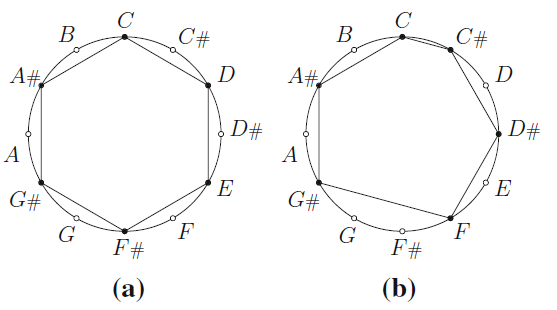
\includegraphics[scale=0.7]{tritone}
\caption{The subsets in a and b represent maximally even scales with and without tritones, respectively}
\end{figure}

The
tritone is defined as a restless interval or dissonance in Western music from the early
Middle Ages. This interval was mostly avoided in medieval ecclesiastical singing
because of its dissonant sound. A maximal antipodal polygon
represents a maximally even set that avoids the tritone

\emph{Odd rythmic patterns}. A rhythm has the rhythmic oddity property if, when
represented on a circle, it does not contain two onsets (the black points in Fig. 3)
that lie diametrically opposite of each other. Note that the property ensures that one
cannot split the circle into two parts of equal length whatever the chosen breaking
onsets is. Thus, these patterns possess a particular type of asymmetry.

\begin{figure}[h!]
\centering
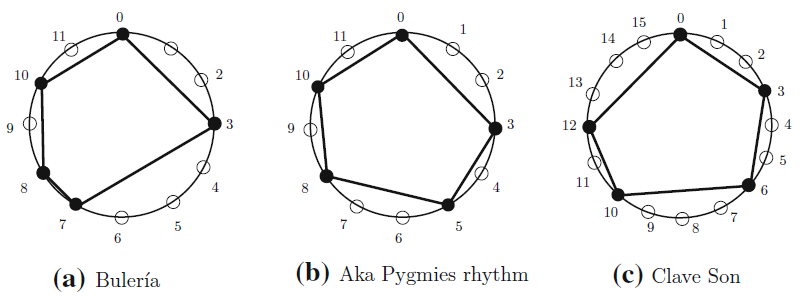
\includegraphics[scale=0.7]{rythm}
\caption{a The bulería rhythm used in Spain, b a rhythm used by the Aka Pygmies of Central Africa, c the
clave son of Cuba}
\end{figure}

They all can be
considered as antipodal polygons with $k < n$ vertices

\subsection{Results}\label{claim}
We will prove the following general result:\\

\emph{Claim} Given an antipodal point set $S ⊂ \R^2$, every thin antipodal polygon on $S$ has
less area than any non-thin antipodal polygon on $S$.\\

In addition we show that the 2-dimensional case is special in the sense that the
above result can not be generalized to higher dimensions.

The analogue result holds for thick antipodal polygons when $n$ is odd but for $n$ even we provide an example of
an antipodal non-thick polygon having larger area than a thick antipodal polygon. However, we are able to prove the following result:\\

\emph{Claim} Given an antipodal point set $S ⊂ \R^2$, for every non-thick antipodal polygon
on $S$ there exists a thick antipodal polygon on $S$ with larger area.\\

Note that above claims imply that an antipodal polygon with minimum (resp. maximum)
area is thin (resp. thick). As a consequence, we will show that the extremal
problems for antipodal polygons can be solved in linear time.

\section{Thin Antipodal Polygons}
Assume that the clockwise circular order of $S$ around the origin is $p_1, p_2, \dots , p_n,
p'_1, p'_2,\dots , p'_n$. For every point $q$ in $S$, let $P_q$ be the thin antipodal polygon that
contains as vertices $q$ and the next $n −1$ clockwise consecutive points of $S$. Note that
all thin antipodal polygons are of this form and that $P_q$ and $P_{q'}$ differ only by a rotation around the origin. 

The next lemma characterizes triangles that contain a given point of S and maximize
the area.

\begin{lem}\label{1}
For a point $p ∈ S$ let $l$ be the line containing $p$ and $p'$. Let $τ$ be the triangle
determined by $p$, and its two neighbors in $S$. Among all triangles that have as vertices
$p$ and one point of $S$ in each of the two half-planes defined by $l$, $τ$ has strictly the
smallest area.
\end{lem}
\begin{proof}
Let $τ'$ be a triangle with vertices in $S$, containing $p$ as a vertex and with a vertex
in each of the two half-planes defined by $l$. Assume that $τ'$ is different from $τ$. Let
$b$ be the side opposite to $p$ in $τ$ and $b'$ be the side opposite to $p$ in $τ'$. Note that $b'$
is at least as large as $b$, because $S$ is an antipodal point set and $l$ contains the origin.
The height of $τ'$ with respect to $p$ is larger than the height of $τ$ with respect to $p$, as
otherwise $b'$ would have to intersect $b$, which is not possible by construction. Thus
the area of $τ'$ is larger than the area of $τ$.

\definecolor{qqqqff}{rgb}{0.,0.,1.}
\definecolor{ffqqqq}{rgb}{1.,0.,0.}
\begin{tikzpicture}[line cap=round,line join=round,>=triangle 45,x=1.0cm,y=1.0cm]
\clip(-3.32,-3.8) rectangle (3.8,3.8);
\fill[line width=1.5pt,color=ffqqqq,fill=ffqqqq,fill opacity=0.6000000238418579] (0.,3.) -- (-1.552610542042701,2.566982762843933) -- (2.141426279814696,2.10102201038423) -- cycle;
\fill[line width=2.pt,color=qqqqff,fill=qqqqff,fill opacity=0.07000000029802322] (0.,3.) -- (-2.844054790410907,-0.9546477618162483) -- (2.141426279814696,2.10102201038423) -- cycle;
\draw [line width=1.pt] (0.,0.) circle (3.cm);
\draw [line width=2.pt,color=ffqqqq] (0.,3.)-- (-1.552610542042701,2.566982762843933);
\draw [line width=2.pt,color=ffqqqq] (-1.552610542042701,2.566982762843933)-- (2.141426279814696,2.10102201038423);
\draw [line width=2.pt,color=ffqqqq] (2.141426279814696,2.10102201038423)-- (0.,3.);
\draw [line width=2.pt,color=qqqqff] (0.,3.)-- (-2.844054790410907,-0.9546477618162483);
\draw [line width=2.pt,color=qqqqff] (-2.844054790410907,-0.9546477618162483)-- (2.141426279814696,2.10102201038423);
\draw [line width=2.pt,color=qqqqff] (2.141426279814696,2.10102201038423)-- (0.,3.);
\draw [line width=1.2pt,dash pattern=on 5pt off 5pt] (0.,3.)-- (0.,-3.);
\draw (-0.16,3.6) node[anchor=north west] {\Large{$p$}};
\draw (-0.24,-3) node[anchor=north west] {\Large{$p'$}};
\draw (0.22,0.4) node[anchor=north west] {\Large{$l$}};
\draw (-0.8,2.85) node[anchor=north west] {\large{$\tau$}};
\draw (-1.,1.56) node[anchor=north west] {\large{$\tau'$}};
\draw [color=ffqqqq](0.16,2.3) node[anchor=north west] {\large{$b$}};
\draw [color=qqqqff](0.4,1.1) node[anchor=north west] {\large{$b'$}};
\begin{scriptsize}
\draw [fill=black] (0.,3.) circle (2.5pt);
\draw [fill=black] (-1.552610542042701,2.566982762843933) circle (2.5pt);
\draw [fill=black] (2.141426279814696,2.10102201038423) circle (2.5pt);
\draw [fill=black] (0.,-3.) circle (2.5pt);
\draw [fill=black] (-2.141426279814696,-2.10102201038423) circle (2.5pt);
\draw [fill=black] (1.552610542042701,-2.566982762843933) circle (2.5pt);
\draw [fill=black] (-2.5618223885561213,1.5611105180263856) circle (2.5pt);
\draw [fill=black] (2.844054790410907,0.9546477618162483) circle (2.5pt);
\draw [fill=black] (2.5618223885561213,-1.5611105180263856) circle (2.5pt);
\draw [fill=black] (-2.844054790410907,-0.9546477618162483) circle (2.5pt);
\end{scriptsize}
\end{tikzpicture}
\end{proof}


We split the proof of the first claim of \ref{claim} into the three cases $n = 3$, $n = 4$, and $n ≥ 5$.

\begin{lem}\label{2}
For $n = 3$, every thin antipodal polygon on $S$ has area strictly less than
that of any non-thin antipodal polygon on $S$.
\end{lem}
\begin{proof}
In this case the only non-thin polygons are the two triangles $τ$ and $τ'$ with vertex
sets $\{p_1, p_2', p_3\}$ and $\{p_1', p_2, p_3'\}$, respectively. Note that $τ$ has the same area as $τ'$.
In addition, by Lemma \ref{1}, $τ$ has larger area than $P_{p_2}$ and $τ'$ has larger area than $P_{p_1}$
and $P_{p_3}$.

\definecolor{qqqqff}{rgb}{0.,0.,1.}
\definecolor{ffqqqq}{rgb}{1.,0.,0.}
\begin{tikzpicture}[line cap=round,line join=round,>=triangle 45,x=1.0cm,y=1.0cm]
\clip(-7.6,-3.7) rectangle (15.4,3.76);
\fill[line width=1.5pt,color=ffqqqq,fill=ffqqqq,fill opacity=0.10000000149011612] (-1.9980473079265573,2.2378129848777437) -- (0.,-3.) -- (2.821128677251516,1.0204082449633143) -- cycle;
\fill[line width=2.pt,color=qqqqff,fill=qqqqff,fill opacity=0.10000000149011612] (-2.821128677251516,-1.0204082449633143) -- (0.,3.) -- (1.9980473079265573,-2.2378129848777437) -- cycle;
\draw [line width=1.pt] (0.,0.) circle (3.cm);
\draw [line width=2.pt,color=ffqqqq] (-1.9980473079265573,2.2378129848777437)-- (0.,-3.);
\draw [line width=2.pt,color=ffqqqq] (0.,-3.)-- (2.821128677251516,1.0204082449633143);
\draw [line width=2.pt,color=ffqqqq] (2.821128677251516,1.0204082449633143)-- (-1.9980473079265573,2.2378129848777437);
\draw [line width=2.pt,color=qqqqff] (-2.821128677251516,-1.0204082449633143)-- (0.,3.);
\draw [line width=2.pt,color=qqqqff] (0.,3.)-- (1.9980473079265573,-2.2378129848777437);
\draw [line width=2.pt,color=qqqqff] (1.9980473079265573,-2.2378129848777437)-- (-2.821128677251516,-1.0204082449633143);
\draw (-2.6,2.68) node[anchor=north west] {\large{$p_1$}};
\draw (0.0,3.6) node[anchor=north west] {\large{$p_2$}};
\draw (3.,1.26) node[anchor=north west] {\large{$p_3$}};
\draw (-3.3,-1.08) node[anchor=north west] {\large{$p_3'$}};
\draw (-0.1,-3.) node[anchor=north west] {\large{$p_2'$}};
\draw (2.,-2.2) node[anchor=north west] {\large{$p_1'$}};
\begin{scriptsize}
\draw [fill=black] (0.,3.) circle (2.5pt);
\draw [fill=black] (0.,-3.) circle (2.5pt);
\draw [fill=black] (-1.9980473079265573,2.2378129848777437) circle (2.5pt);
\draw [fill=black] (2.821128677251516,1.0204082449633143) circle (2.5pt);
\draw [fill=black] (1.9980473079265573,-2.2378129848777437) circle (2.5pt);
\draw [fill=black] (-2.821128677251516,-1.0204082449633143) circle (2.5pt);
\end{scriptsize}
\end{tikzpicture}
\end{proof}


\begin{lem}\label{3}
For $n = 4$, every thin antipodal polygon on $S$ has area strictly less than
that of any non-thin antipodal polygon on $S$.
\end{lem}


\begin{thm}
Every thin antipodal polygon on $S$ has less area than any non-thin antipodal
polygon on $S$.
\end{thm}

The idea of the proof is induction on $n$ with lemmas \ref{2} and \ref{3} as base case. For $n\geq 5$, consider a triangulation $T$ of $S$, and by analysing the thin triangles of $T$ one can reduce the problem to the case $n-1$. 


\section{Thick Antipodal Polygons}
ULISES

\section{Higher Dimensions: Antipodal Polytopes}
ULISES


 \section{Open Problems}
 
 %CIRCULAR LATTICE ES UN CÍRCULO CON PUNTOS IGUALMENTE ESPACIADOS 
Let us assume that we are given a circular lattice with an antipodal set of $2n$ points
(evenly spaced) and we would like to compute an extremal antipodal $k$-polygon with
$k < n$ vertices. For $k = n$, the linear algorithms proposed in this paper are strongly based on
the simple characterization for the extremal antipodal polygons. Namely, the minimal
thin antipodal polygon has consecutive vertices and the thick antipodal polygon has
an alternating configuration. That
characterization does not hold in the general case $k < n$.


\definecolor{zzttqq}{rgb}{0.6,0.2,0.}
\begin{tikzpicture}[line cap=round,line join=round,>=triangle 45,x=1.0cm,y=1.0cm]
\clip(-6.246666666666667,-2.066666666666644) rectangle (9.086666666666668,2.07);
\fill[line width=2.pt,color=zzttqq,fill=zzttqq,fill opacity=0.10000000149011612] (-1.7557911458287687,0.9577042613611466) -- (0.,2.) -- (1.0229677195353655,1.7185857688194133) -- (1.755791145828769,0.9577042613611464) -- (2.,0.) -- cycle;
\draw [line width=1.2pt] (0.,0.) circle (2.cm);
\draw [line width=2.pt,color=zzttqq] (-1.7557911458287687,0.9577042613611466)-- (0.,2.);
\draw [line width=2.pt,color=zzttqq] (0.,2.)-- (1.0229677195353655,1.7185857688194133);
\draw [line width=2.pt,color=zzttqq] (1.0229677195353655,1.7185857688194133)-- (1.755791145828769,0.9577042613611464);
\draw [line width=2.pt,color=zzttqq] (1.755791145828769,0.9577042613611464)-- (2.,0.);
\draw [line width=2.pt,color=zzttqq] (2.,0.)-- (-1.7557911458287687,0.9577042613611466);
\begin{scriptsize}
\draw [fill=black] (0.,0.) circle (1.5pt);
\draw [fill=black] (0.,2.) circle (2.0pt);
\draw [fill=black] (-1.0229677195353652,1.7185857688194135) circle (2.0pt);
\draw [fill=black] (-1.7557911458287687,0.9577042613611466) circle (2.0pt);
\draw [fill=black] (-2.,0.) circle (2.0pt);
\draw [fill=black] (0.,-2.) circle (2.0pt);
\draw [fill=black] (1.0229677195353652,-1.7185857688194135) circle (2.0pt);
\draw [fill=black] (1.7557911458287687,-0.9577042613611466) circle (2.0pt);
\draw [fill=black] (2.,0.) circle (2.0pt);
\draw [fill=black] (1.0229677195353655,1.7185857688194133) circle (2.0pt);
\draw [fill=black] (1.755791145828769,0.9577042613611464) circle (2.0pt);
\draw [fill=black] (-1.755791145828769,-0.9577042613611464) circle (2.0pt);
\draw [fill=black] (-1.0229677195353655,-1.7185857688194133) circle (2.0pt);
\end{scriptsize}
\end{tikzpicture}

Finding the
extremal antipodal $(n−1)$-polygon, called $(2n, n−1)$-problem for short, can be easily
reduced to solve $O(n)$ times the $(2(n − 1), n − 1)$-problem: in the $(2n, n − 1)$-problem an antipodal pair is not selected and can thus be removed
from the input. This approach gives a simple $O(n^{n−k+1})$ time algorithm for solving
the general $(2n, k)$-problem. This leaves the open question if the $(2n, k)$-problem can
be solve in $O(n^k )$ time.
\end{document}
